\chapter{Landscape Analysis and Representation}


\section{Reviewing}
\begin{enumerate}
\item
For ResNet, what should be the right initialization?

$\beta$-scaling: scale the variance of the weight matrix $W$ by $1/L$.
\begin{remark}
Summarization for initialization tricks of the weight matrix $W^{\ell}$:
\begin{itemize}
\item
Gaussian random $W^{\ell}$
\item
Orthogonal $W^{\ell}$
\item
For $W^{\ell}$ of the form $\text{Identity}+\text{Gaussian matrix }H$, scale the variance of the Gaussian matrix by $1/L$.
\end{itemize}
\end{remark}
\begin{remark}
The insights behind the hw1, question~5 are close to the initialization tricks for ResNet.
In order to gurantee $\|z^{L}\|/\|x\|=\mathcal{O}(1)$, the trick for the ResNet is to make $\mathbb{E}[(I+H)^L]=\mathcal{O}(I)$;
In order to gurantee $\mathbb{E}[\|Wx\|^2]=\mathbb{E}[\|x\|^2]$, it suffices to make $\mathbb{E}[WW\trans]=I$, or more specifically, 
\begin{itemize}
\item
$W$ and $x$ are independent;
$W_{i,j}$'s are independent;
\item
$\mathbb{E}W_{i,j}=0,\forall i,j$;
$\sum_j\mathbb{E}(W_{i,j}^2)=1$.
\end{itemize}

\end{remark}
\item
When does the non-convexity not scary?

When the objective funciton has no sub-optimal local minima, i.e., 
each second order stationary point is global minima.
\item
Under which condition, 
a deep neurel-net loss function has no sub-optimal local minima?
\begin{itemize}
\item
Mutli-layer is not an issue.
\item
Most non-linear activation functions seems not an issue;
However, for ReLU function, there do exists sub-optimal local minima.
Therefore, the non-linearity sometimes does cause an issue.
\end{itemize}

\end{enumerate}

\paragraph{Outline}
\begin{itemize}
\item
Non-linear neural-nets landscape analysis
\item
Universal Approximation Theorem
\end{itemize}


\section{
Landscape analysis for non-linear neural-nets
}
\subsection{Negative Result: 
The sum of two good-landscape function have good landscape
}
A function with good-landscape means that there exists sub-optimal local minima.
It's reasonable to think that the sum of two good-landscape function has a good landscape, since convex functions have good landscape, and the convexity holds under summation.

Unfortunately, 
the paper \citep{NIPS19951028} gives counter-examples for this statement.
Consider the error functions 
\[
E_1(w)=(y_1 - \phi(wx_1))^2,\qquad
E_2(w)=(y_2 - \phi(wx_2))^2,
\]
then it's possible that the error function $E\triangleq E_1+E_2$ contains the local minimas of $E_1$ and $E_2$. In this way more local minimas can be produced, which may lead to bad landscape.
\begin{figure}[H]
\centering
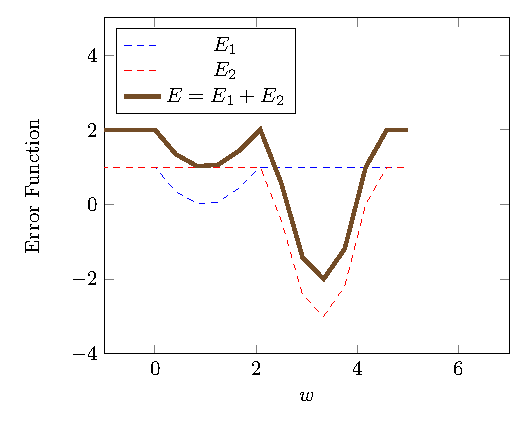
\includegraphics[width=0.7\textwidth]{Sixth_lecture/f_3}
\caption{Illustraion of a counter-example for $1$-dimension case}
\label{fig:6:1}
\end{figure}
We made the assumption that the loss function is bounded\footnote{but ReLU does not satisfy this assumption}, then the paper \citep{NIPS19951028} further shows that the number of local minima of the error function grows can grow exponentially in the dimension. 
\begin{theorem}[Theorem 3.4 in \citep{NIPS19951028}]
Let $\phi$ and $\ell(\cdot,\cdot)$ satisfy the assumption;
then for all $n\ge1$, there exists data $\{(x_i,y_i)\}_{i=1}^n$ such that 
\[
F(w) = \frac{1}{n}\sum_{i=1}^n\ell(y_i,\phi(wx_i))
\]
has $\lfloor n/d\rfloor^d$ distinct local minima.
\end{theorem}
This seems a negative result, but we consider adding some extra conditions to make it positive.
First introduce the notion of \emph{minimum-containing} set:
\begin{definition}
Let $f:\mathbb{R}^d\to\mathbb{R}$ be a continuous function. 
Then an open and bounded set $U\in\mathbb{R}^d$ is called a \emph{minimum-containing} set for $f$ 
if for each $w$ on the boundary of $U$, there
is a $w^*\in U$ such that $f(w^*)<f(w)$.
\end{definition}
Graphically speaking, the minimum-containing set for a loss function is its ``hole'' part. In Fig.~\ref{fig:6:1} we can see that $E_1$ and $E_2$ has different holes, which makes $E$ has two distinct holes, which results in two distinct local minima.

The question is that does this phenomena happen frequently? In other words, is it possible to add mild (practical) conditions to eliminate extra \emph{minimum-containing} set?

\begin{theorem}[Theorem 5.1 in \citep{NIPS19951028}]
Let $\phi$ and $\ell$ satisfy the previous condition, and further assume that $\phi$ is monotone and $\ell$ is qusi-motonone, i.e., $L(y,y+r_1)\le L(y,y+r_2)$ for $0\le r_1\le r_2$ or $r_2\le r_2\le0$.
Given a sequence of data $\{(x_i,y_i)\}_{i=1}^n$, assume that there exists parameter $w$ such that $\phi(wx_i)=y_i$ for all $i$. As a result, there is only one minimum-containing set in the loss function $F(w)$.
\end{theorem}

\begin{remark}
In the $1$-layer neural net with non-linear activation, we can see that the loss function has a good landscape only if each dataset is \emph{realizable}
\footnote{This condition is recently also called the interpolation property}, i.e., there exists parameter $w$ such that $\phi(wx_i)=y_i$.
The intuition is that in this case each component of the loss function share the same minimizer $w^*$. 
Therefore, the necessary condition for a loss function to have a good landscape is that representation power of the neural net is ``enough''.
\end{remark}


\section{Over-Parameterized Networks}
It's a common sense that deep~(over-parameterized) networks are effiective descriptors for our physical world.
However, it requires long computation time, large storage space and otherwise.
Due to the limited resource, it is popular to do the network pruning of a large network to get a reasonable effiective descriptor.
See \citep{frankle2018the} and \citep{NIPS2015_5784} for related work.
\begin{center}
\smartdiagramset{back arrow disabled=true,
text width=1.5cm
}
\smartdiagram[flow diagram:horizontal]{
Train,
Network Pruning,
Fine-Tuning
}
\end{center}
However, it is not effiective to train a small network directly.
One possible reason is that bigger networks may have better landscape.
The evidence is that training larger network is in general ``easier'' than smaller one in practice.

\paragraph{Does Current Neural-net have too many parameters?}
This is not clearly understood now.
Prof. Ruoyu Sun makes an analogy from the function fitting example.
To fit an underlying function $\mathbb{R}^d\to\mathbb{R}$ given $n$ samples, tuning $n$ parameters are enough.
However, to fit an underlying function $\mathbb{R}^d\to\mathbb{R}^{d_y}$ given $n$ samples, it seems at least we need $n\cdot d_{y}$ samples.
From this analogy, we infer that given $n$ samples, each layer has $n$ degree of freedom, and we call the phenomena that, training neural network with more than $n$ neuros each layer, the \emph{over-parametrization}.

\paragraph{Bibliography}
There are three classical works on the over-parametrization issue of neural networks before 2000.
The paper \citep{BALDI198953} simply shows that the landscape for the loss function of $1$-hidden layer linear neural network is good;
following this work, however, the paper \citep{NIPS19951028} shows that adding non-linearity activation can create many bad local minima;
suprisingly, \citep{410380} shows that under the assumption of over-parametrization, $1$-hidden layer nonlinear neural network has good landscape. However, Prof. Ruoyu Sun claims that the statement from this paper is wrong. He gives extension work in \citep{ruoyusun2018}.

Let's discuss the work \citep{410380} in detail. Consider quadratic loss for $1$-hidden layer nonlinear neural network under the assumption that the number of hidden neuron in each layer is more than the number of samples:
\[
\min_{W_1,W_2}\|Y - W_2\sigma(W_1X)\|_F^2
\]

To understand thir work, define the following properties:
\begin{itemize}
\item
Property [PT]: Starting from any initial point, there exists a \emph{small} perturbation $\Delta$ and a strictly decreasing path from $\theta+\Delta$ to a global minima
\item
Property [P]: Starting from any initial point, there exists a strictly decreasing path from $\theta$ to a global minima, which further implies that there is no bad sub-optimal local minima.
\end{itemize}
Their work essentially shows the over-parameterized problem has the property [PT] instead of the property [P]. The paper \citep{ruoyusun2018} is the first one that finds this mistake.
We can easily see that hte property [PT] does not necessarily imply no bad local minima exist by considering the counter-example in the Figure~\ref{fig:6:2}.

In fact, the property [PT] only implies that 
no suboptimal strict local minimum exists, but suboptimal local minima can possibly exist.
We say the existence of strict local minimum as the existence of bad basin:
\begin{figure}[H]
\centering
\begin{minipage}[t]{0.48\textwidth}
\centering
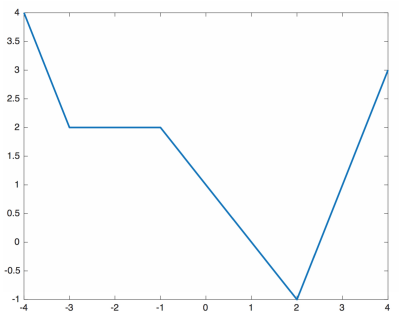
\includegraphics[width=\textwidth]{Sixth_lecture/f_5.png}
\caption{No bad basin}
\label{fig:6:2}
\end{minipage}
\begin{minipage}[t]{0.48\textwidth}
\centering
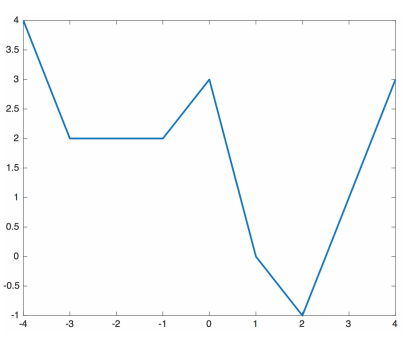
\includegraphics[width=\textwidth]{Sixth_lecture/f_6.png}
\caption{Example of bad basin}
\label{fig:6:3}
\end{minipage}
\end{figure}

What we really need to worry about is the existence of bad basin in our loss function, i.e., exitence of strict local minima. However, such cases are rara in neural-nets due to its symmetry. For instance, matrix factorization is one of the cores in the deep learning training:
\[
\min_{X,Y}\|A-XY\|_F^2
\]
As long as we pick the solution pair $(X,Y)$, the solution pair $(XT,T^{-1}Y)$ admits the same objective value for any orthogonal matrix $T$.

\subsection{Empirical Evidence for Landscape}
There is some evidence that large neural nets have nice landscape, but whether it is true, or how this can help us design better netowkr are still open problems.
Since these results are empirical, the details are skipped, but only few works are listed.
\paragraph{Bibliography}
The paper \citep{43404} examines that, on a straight path from initialization to solution, a variety of state-of-the-art neural networks never encounter any significant obstacles~(basins).
The paper \citep{NIPS2018_8095} and \citep{Gotmare2018} empirically finds that the optima of  neural network loss functions are connected by simple curves over which training and test
accuracy are nearly constant, which is called the \emph{Mode Connectivity} phenomena.
These empirical findings may potentially help us understand the landscape of loss functions, and the insights for robustness during training. 

\begin{remark}
\begin{enumerate}
\item
The landscape for large neural network is nice, but it is not the case where each local-minima is global minima.
\item
It would be helpful to analysis the landscape from geometric point of view, and we hope to generalize the empirical findings to theory.
\item
There are recent results in other applications of neural network, such as reinforcement learning (Google Brain is working on it), GAN \citep{DBLPkarol}, and otherwise.
\end{enumerate}


\end{remark}



\section{Representation Power}
Finally, we give some quick introduction to the representation power of neural network.

\paragraph{Motivation}
Suppose we have a bunch of points in a unit square, and we have two classes, inside the circle is class one, outside the circle is class two.
The goal is to build a classifier to classify these two classes, then it is never possible to apply linear classifier to get positive results, since linear classifier does not have strong representation power.
We can formalize the notion of representation power with math.
\paragraph{Formulation of Representation Power}
\begin{itemize}
\item
Given a target domain $\mathcal{D}\subseteq\mathbb{R}^d$, which is usually assumed to be \emph{compact}.
For simplicity suppose that $\mathcal{D}=[0,1]^d$.
\item
Given a target function $f(x)\in\mathcal{C}(\mathcal{D})$.
\item
Given a candidate family $\mathcal{F}$:
\begin{align*}
\mathcal{F}&=\{
f\mid 
f=v\trans\phi(wx+b),
v\in\mathbb{R}^{1\times m},
w\in\mathbb{R}^{m\times b},b\in\mathbb{R}^m,
\text{some }m\in\mathbb{N}
\}\\
&=\text{span}\{
\phi(\inp{w}{x}+w_0), w\in\mathbb{R}^{d},w_0\in\mathbb{R}
\}
\end{align*}
\item
We say that $\mathcal{F}$ represents $f$ if for any $\varepsilon$, there exists $f\in\mathcal{F}$ such that $\|f-g\|\le\varepsilon$. In other words, the candidate family $\mathcal{F}$ has \emph{enough representation power} w.r.t. the target function $f$.
\end{itemize}

\paragraph{Sufficient Condition for Enough Representation Power}
Few sufficient conditions given for building the enough representation power of $F$:
\begin{itemize}
\item
When $\phi(\cdot)$ is a bounded, non-constant and continuous function, then $\mathcal{F}$ can represent any continuos mapping $f$  \citep{Hornik1991}.
\item
If $\phi(\cdot)$ is bounded, non-constant,
then $\mathcal{F}$ can represent any function $f$ in $\mathcal{L}^p(\mu)$. (see Stone-Weierstrass Theorem for detail in real analysis note \citep{jiewang2019}).
\item
ReLU is not a bounded function, but we can still show that the ReLU activation has enough representation power by some easy-following argument.
\end{itemize}

In next lecture, we will give some introduction to GAN.












